\documentclass{jsarticle}
\usepackage{graphicx,listings}
\lstset{language={C},%
  basicstyle=\footnotesize,%
  commentstyle=\textit,%
  classoffset=1,%
  keywordstyle=\bfseries,%
  frame=tRBl,framesep=5pt,%
  showstringspaces=false,%
  numbers=left,stepnumber=1,numberstyle=\footnotesize%
}%


\title{情報実験第三 1.C}

\author{情報工学科15\_03602 柿沼 建太郎 \\ 情報工学科 15\_10588 中田 光}
\date{\today}
\begin{document}
\maketitle

\section*{各課題担当者}
各課題と担当者を表として以下に示す。
\begin{table}[h]
\begin{tabular}{|l|c|c|} \hline
課題番号/名前 & 柿沼 & 中田 \\ \hline \hline
素数プログラム &  & $\circ$ \\ \hline
test\_calc1 & $\circ$ & \\ \hline
test\_io2 & $\circ$ & $$ \\ \hline
\end{tabular}
\end{table}

\newpage

\section*{FPGA実装レポート}

\subsection*{課題1. 素数プログラムにN以下の素数を全て出力する機能を追加し、FPGAで動作検証する}
担当:中田\\

\subsubsection*{概要}
以前作成した素数プログラムをもとに作成した。アルゴリズムは課題1.Aと同様で与えられたNに対し
それ以下の全ての自然数に除算を行うことで判定している。\\
入力Nは16進の4桁とし、出力はN以下の素数を空白ごとに10進数で出力している。Nを入力しENTERを押すと結果が出力される。\\
\\
※FFFFは実行時間が膨大になると考えられたので途中で中断した実行結果である。


\subsubsection*{実行結果}


\begin{figure}[htbp]
 \begin{minipage}{0.5\hsize}
  \begin{center}
  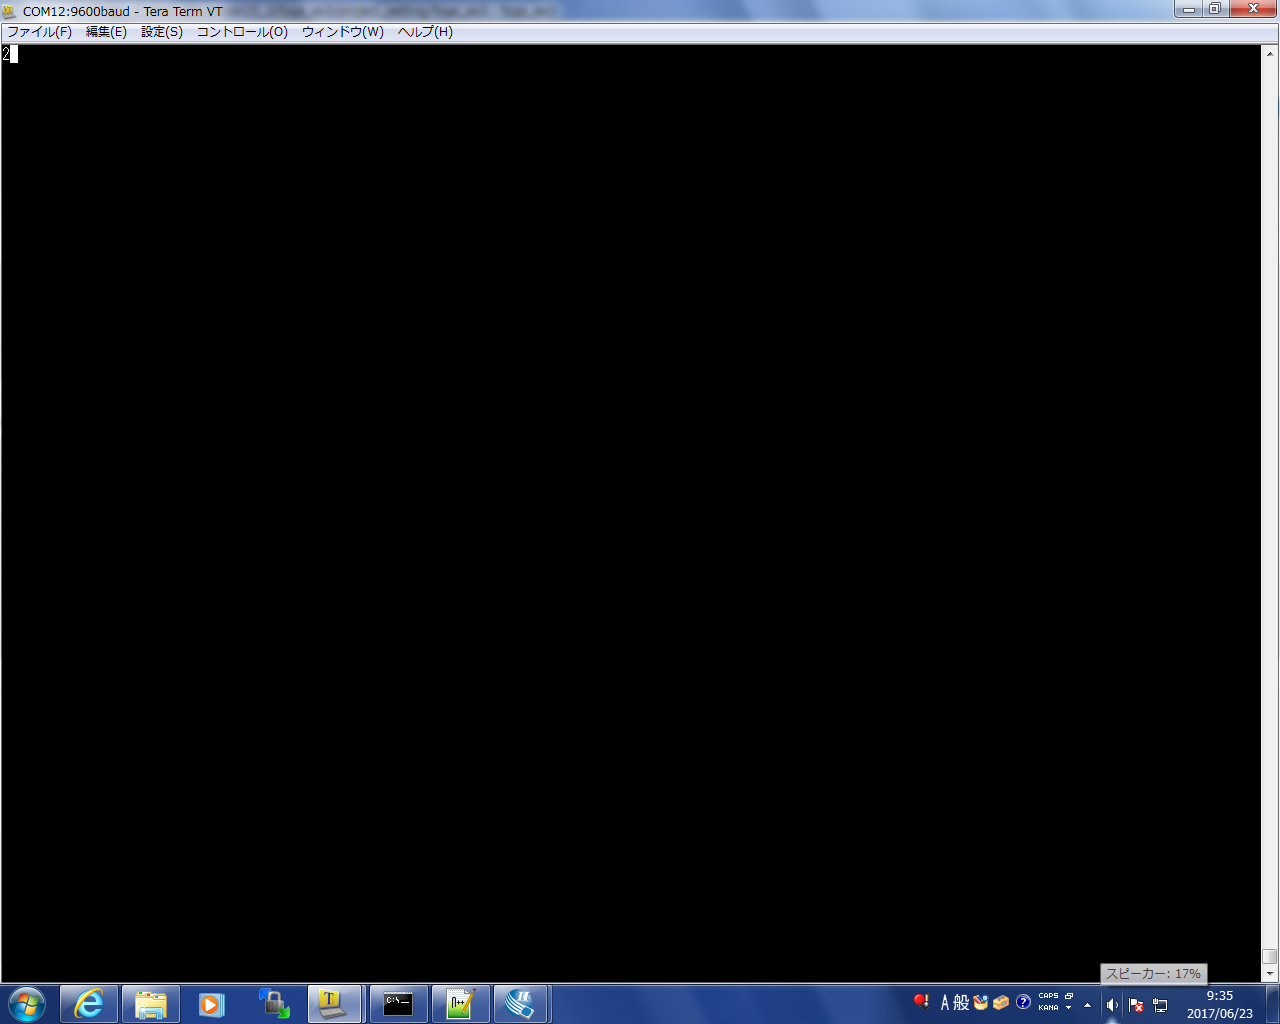
\includegraphics[width=8cm,bb=0 0 1280 1024]{2out.png}
  \end{center}
  \caption{"2"}
 \end{minipage}
 \begin{minipage}{0.5\hsize}
  \begin{center}
   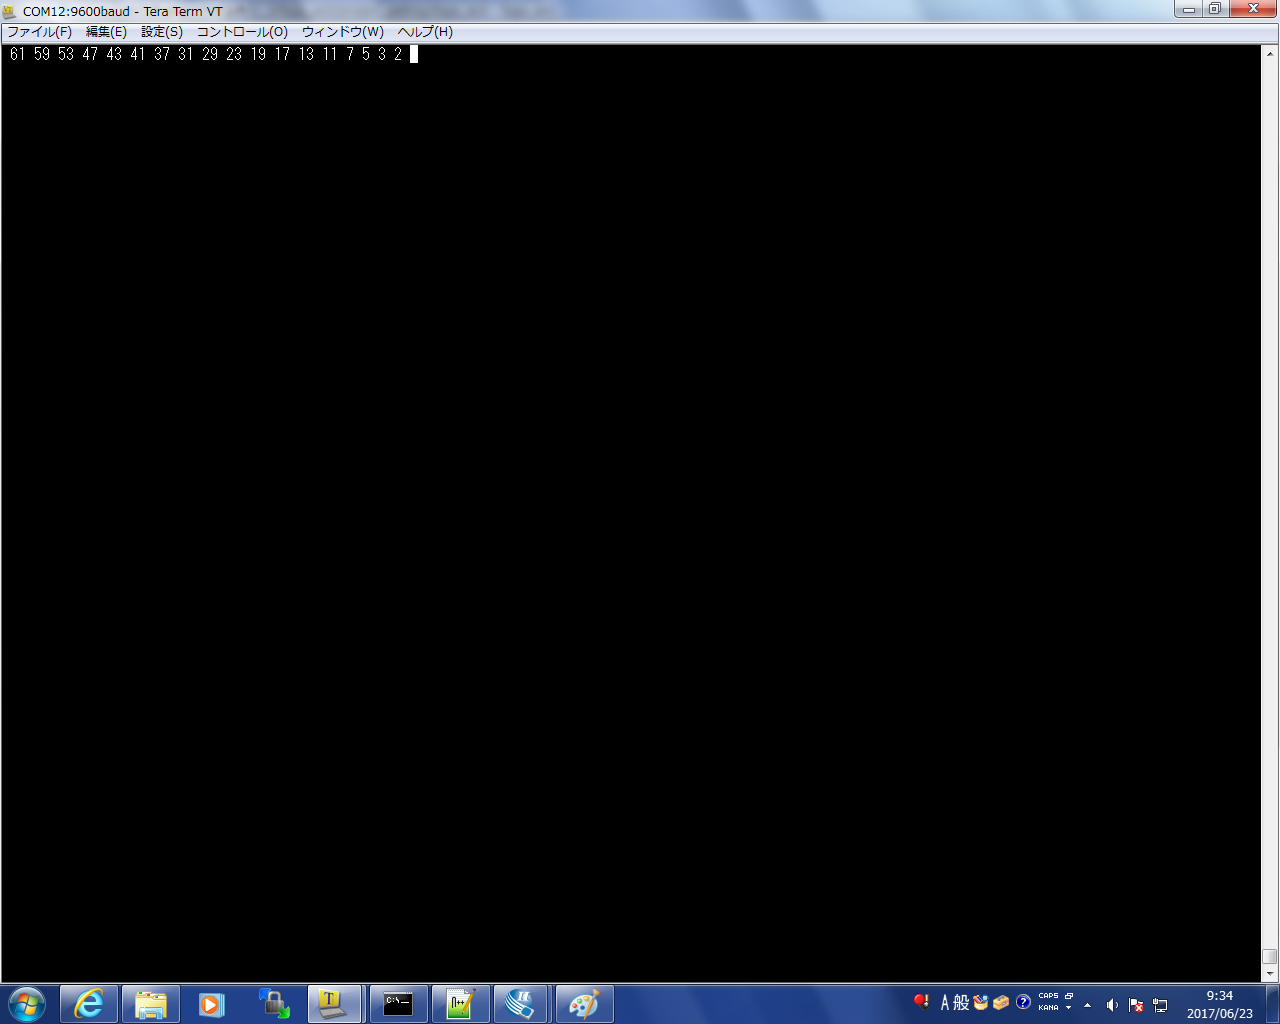
\includegraphics[width=8cm,bb=0 0 1280 1024]{40out.png}
  \end{center}
  \caption{"40"}
 \end{minipage}
\end{figure}

\begin{figure}[htbp]
 \begin{minipage}{0.5\hsize}
  \begin{center}
  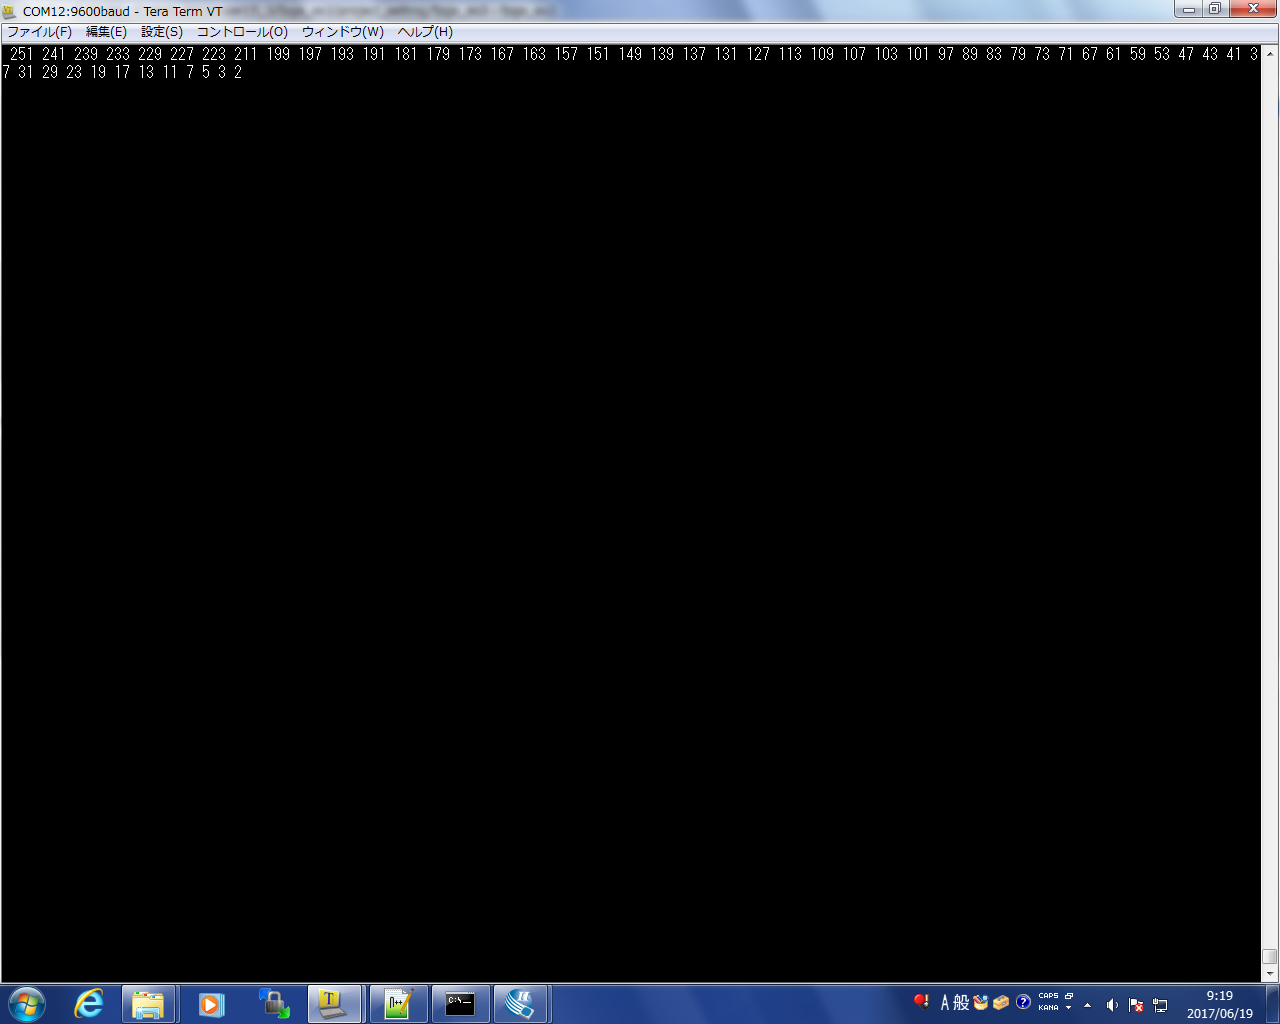
\includegraphics[width=8cm,bb=0 0 1280 1024]{FFout.png}
  \end{center}
  \caption{"FF"}
 \end{minipage}
 \begin{minipage}{0.5\hsize}
  \begin{center}
   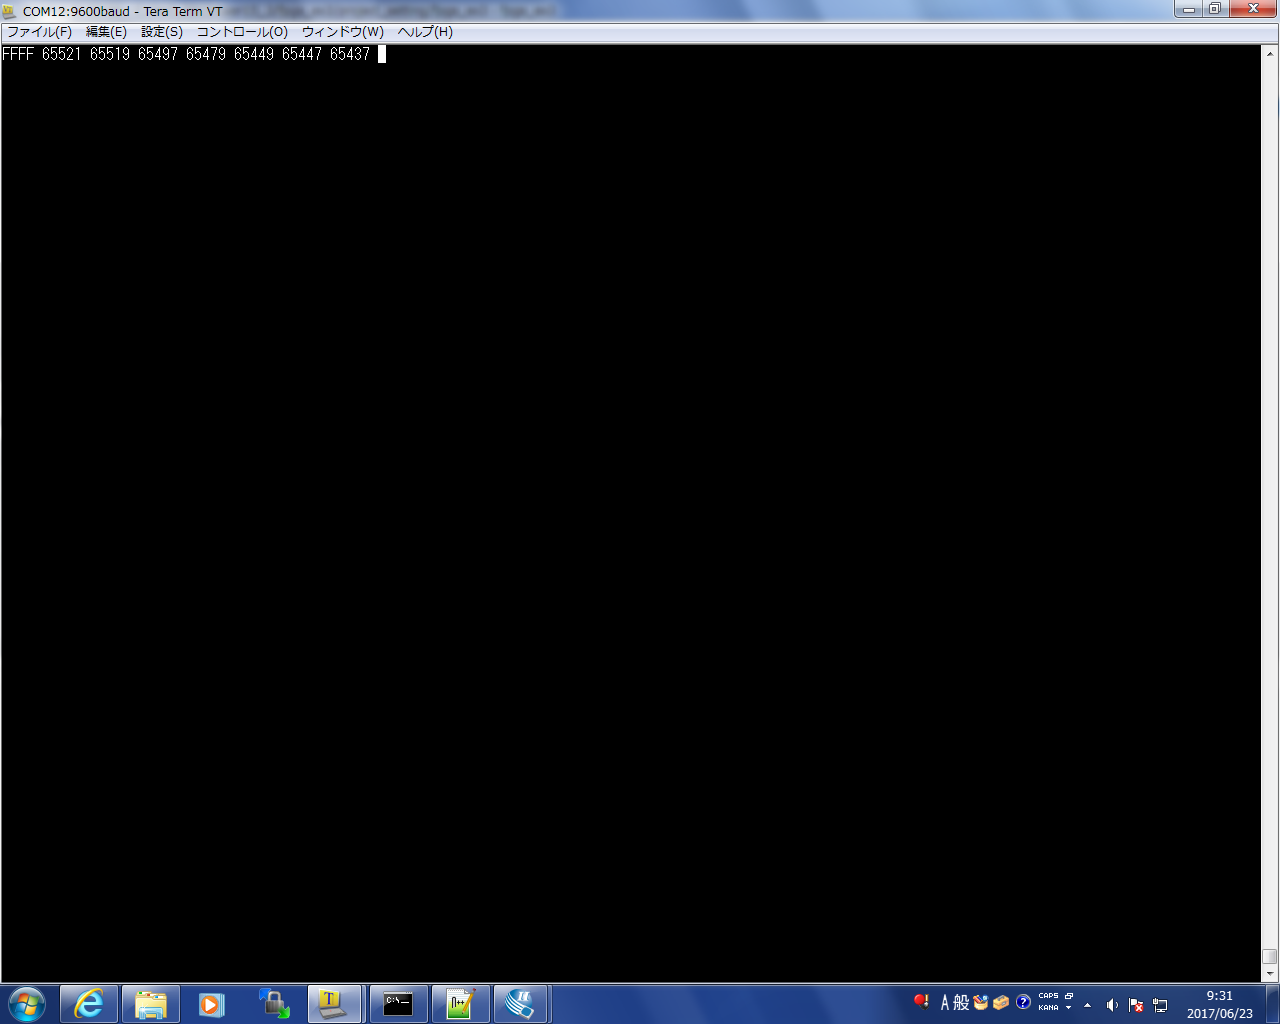
\includegraphics[width=8cm,bb=0 0 1280 1024]{FFFFinout.png}
  \end{center}
  \caption{"FFFF"}
 \end{minipage}
\end{figure}

\newpage

\subsubsection*{ソースコード}

\lstinputlisting[caption=素数プログラム]{./report1_4_nakata_verilog3.asm}


\newpage


\subsection*{課題2.test\_calc1の計算結果を7セグメントディスプレイに表示するように改良し、FPGAで動作検証する}
担当:柿沼\\
\subsubsection*{概要}

\subsubsection*{実行結果}

\begin{figure}[htbp]
 \begin{minipage}{0.5\hsize}
  \begin{center}
  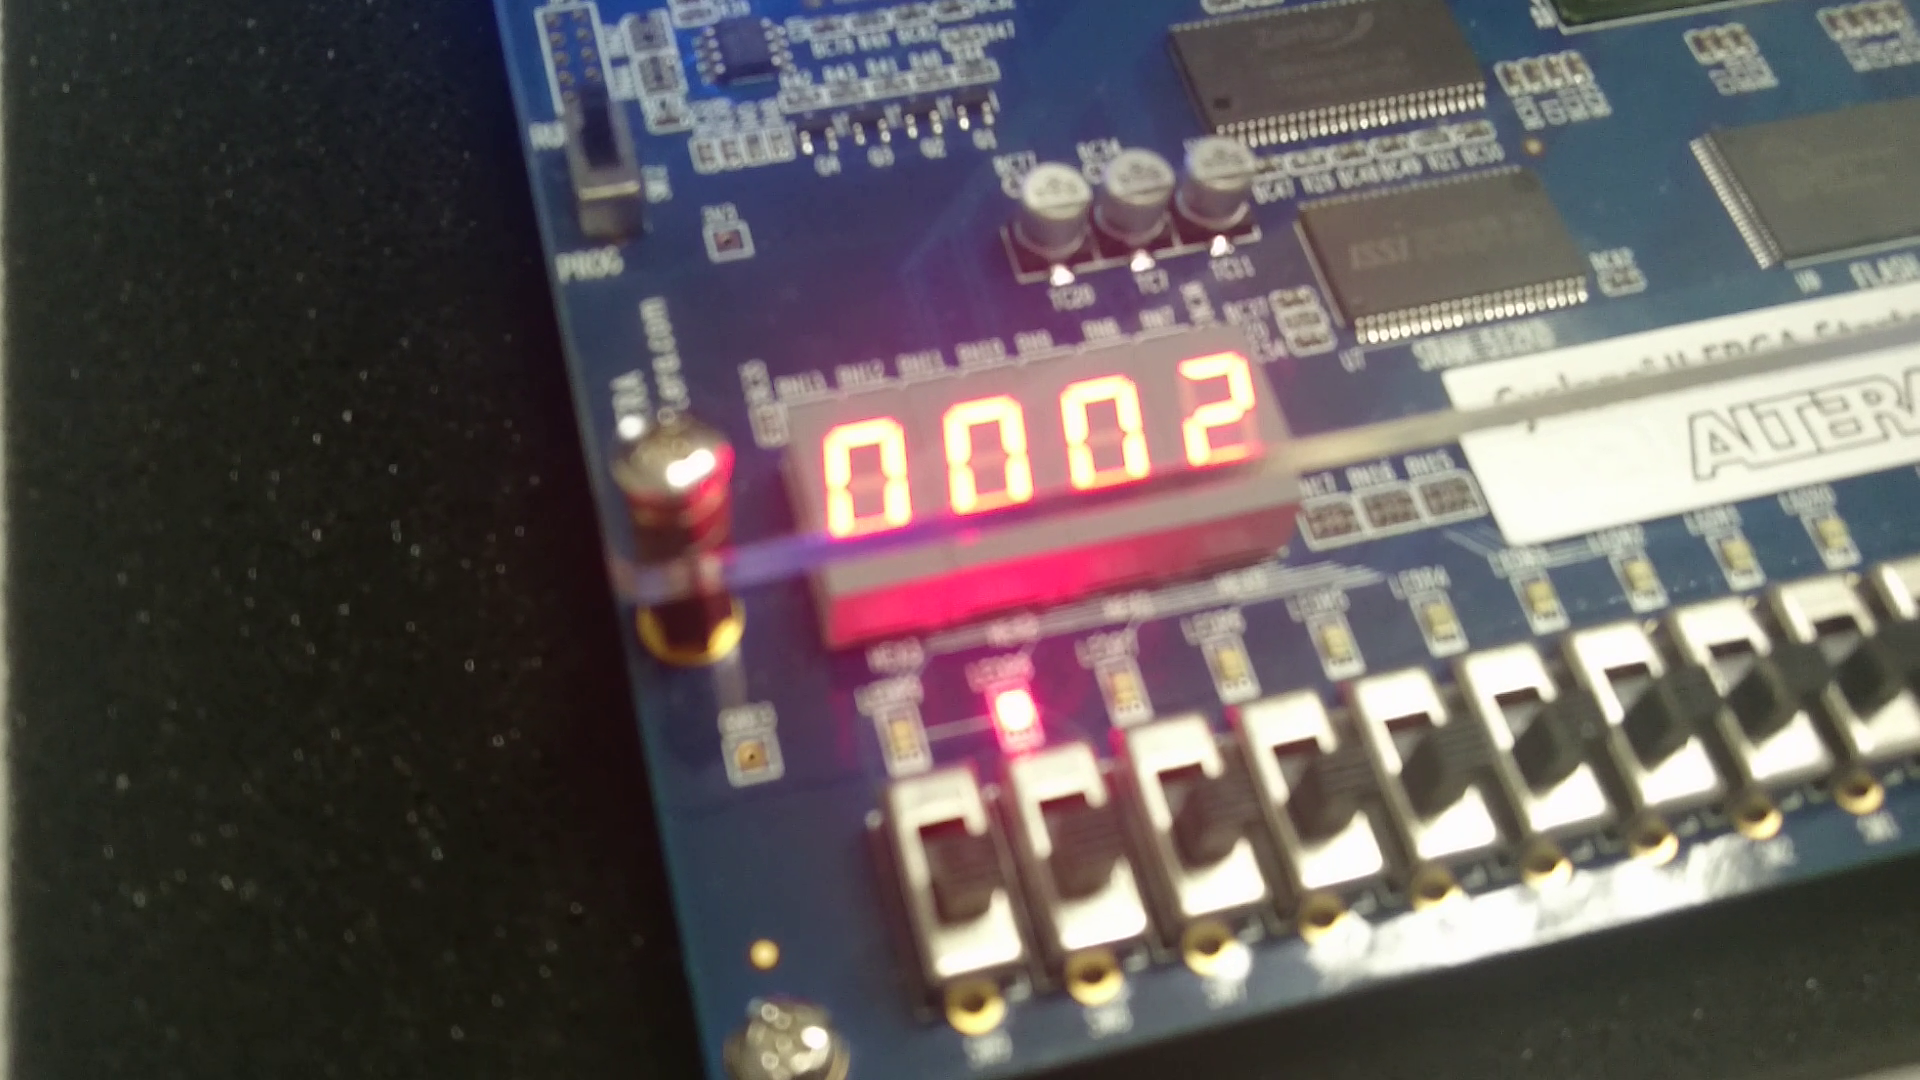
\includegraphics[width=8cm,bb=0 0 1920 1080]{1+1.png}
  \end{center}
  \caption{"1+1="}
 \end{minipage}
 \begin{minipage}{0.5\hsize}
  \begin{center}
   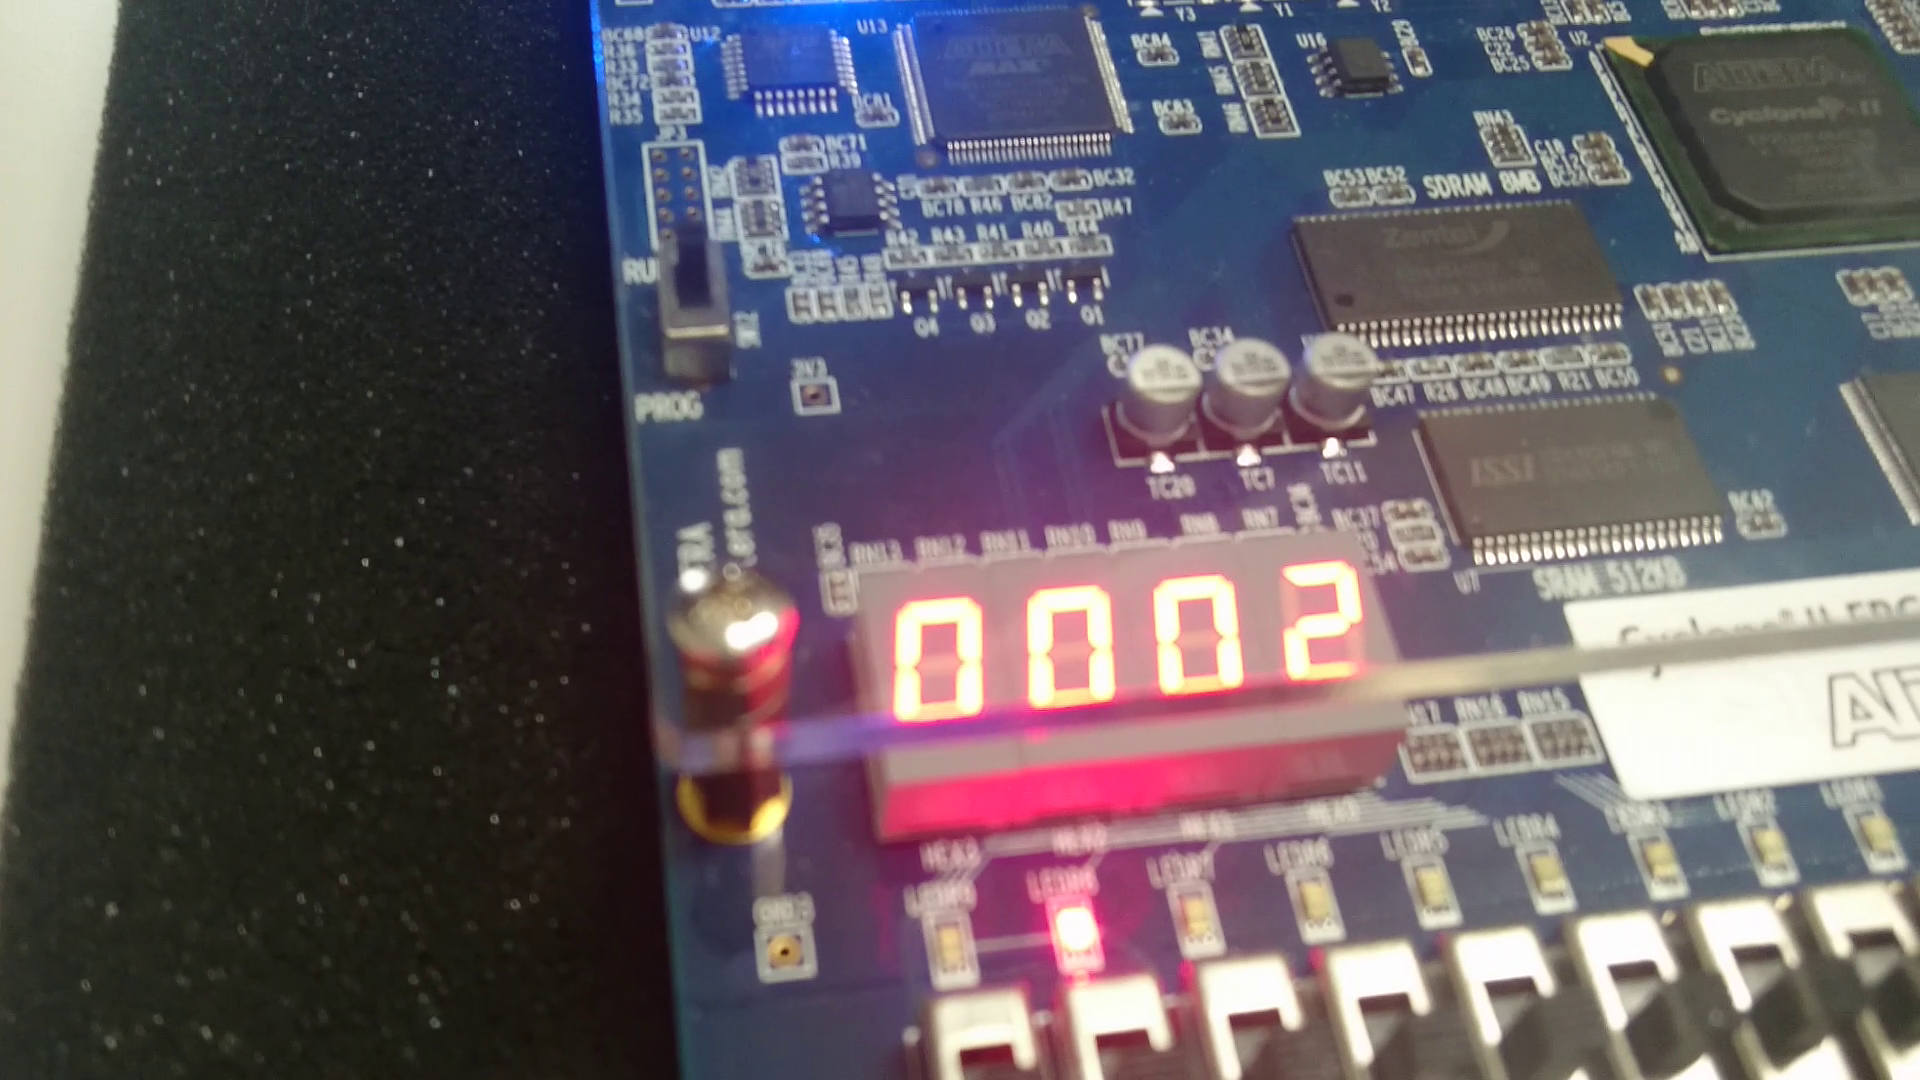
\includegraphics[width=8cm,bb=0 0 1920 1080]{3-1.png}
  \end{center}
  \caption{"3-1="}
 \end{minipage}
\end{figure}

\begin{figure}[htbp]
 \begin{minipage}{0.5\hsize}
  \begin{center}
  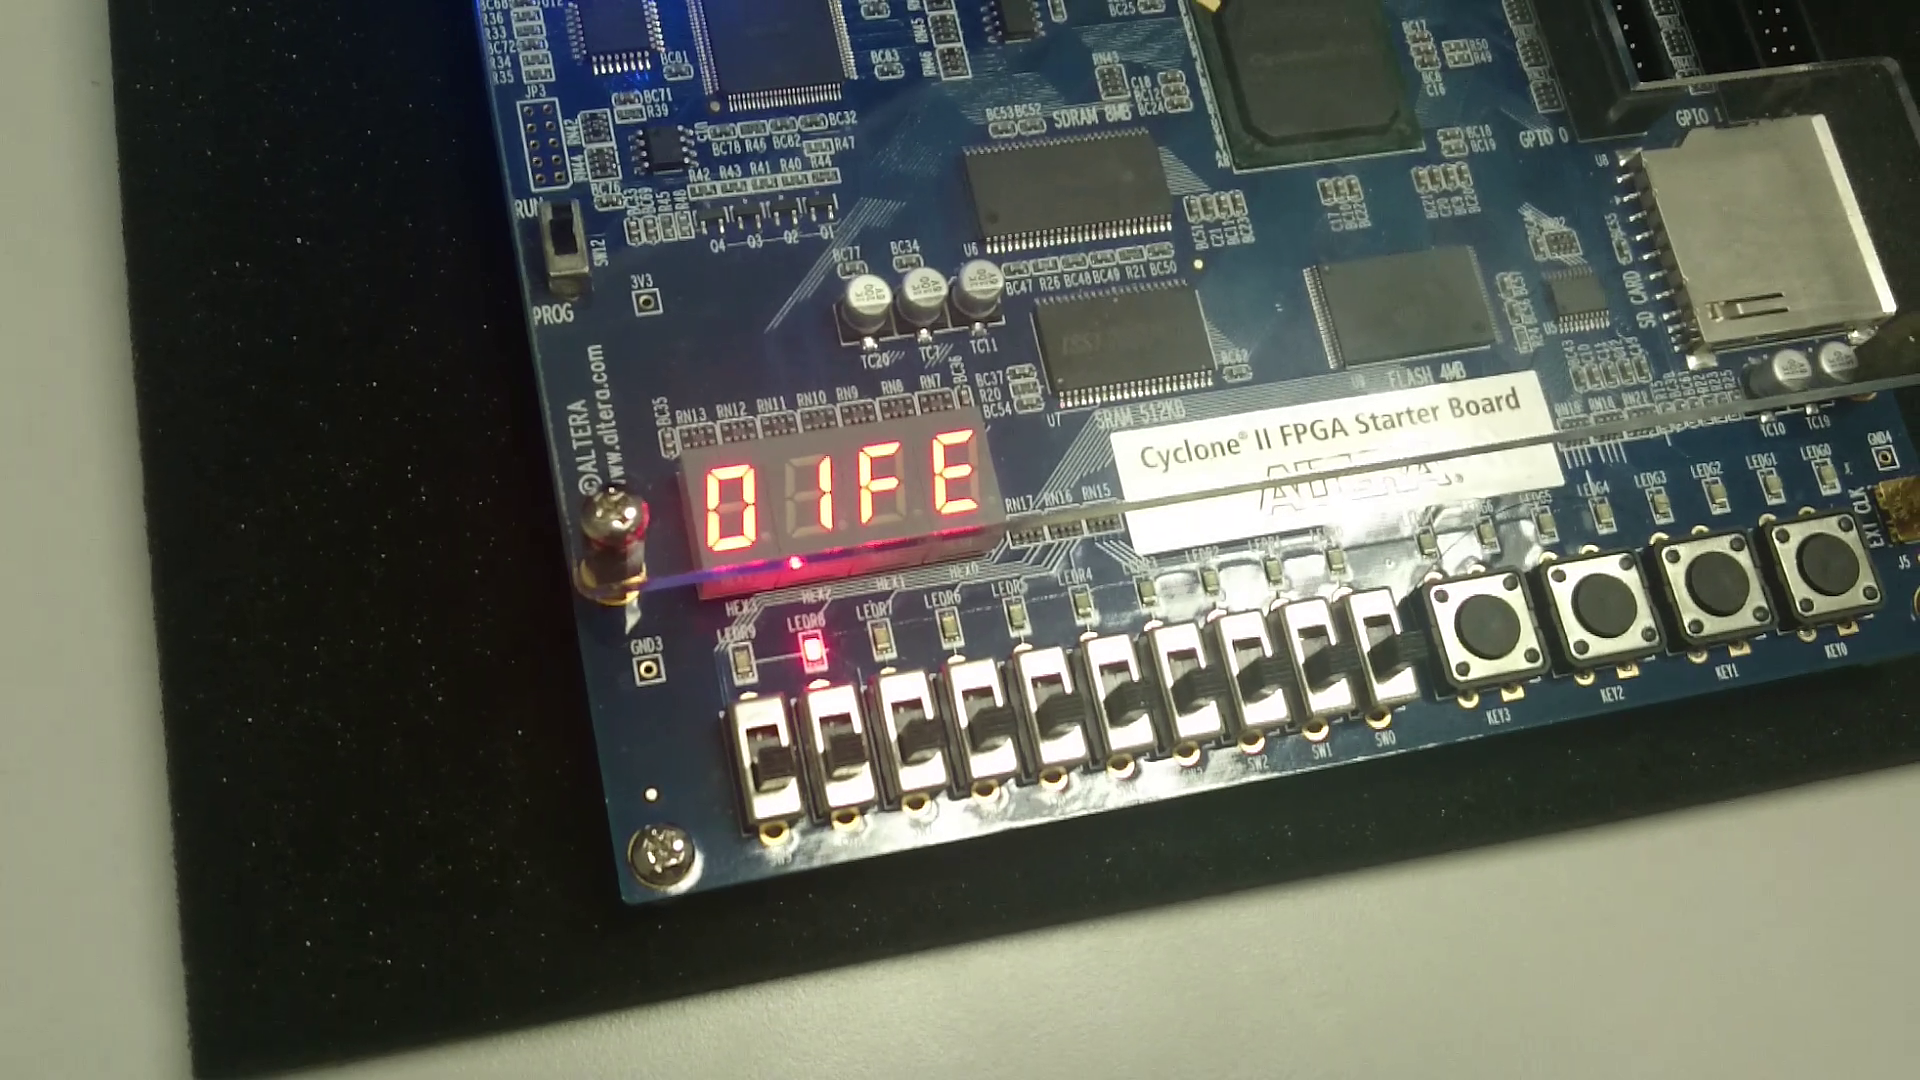
\includegraphics[width=8cm,bb=0 0 1920 1080]{FF+FF.png}
  \end{center}
  \caption{"FF+FF="}
 \end{minipage}
 \begin{minipage}{0.5\hsize}
  \begin{center}
   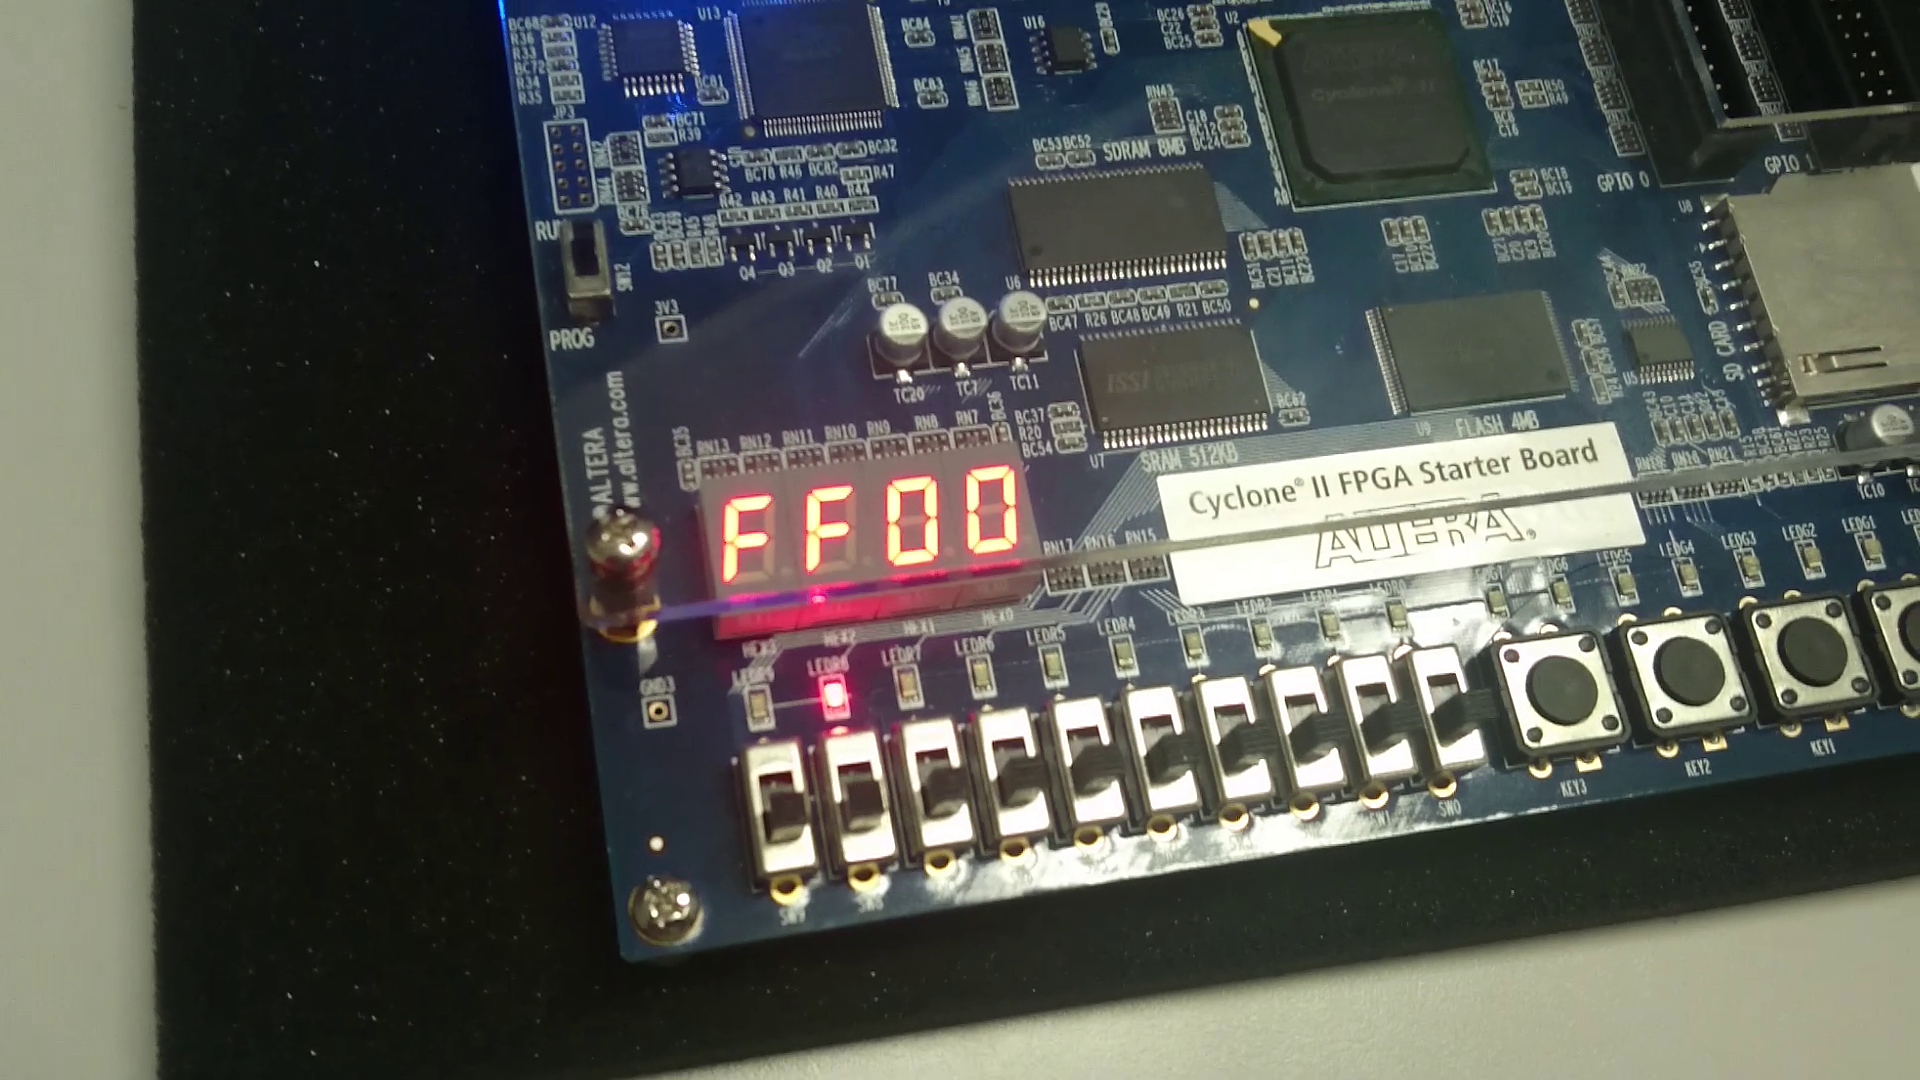
\includegraphics[width=8cm,bb=0 0 1920 1080]{FFFF-FF.png}
  \end{center}
  \caption{"FFFF-FF="}
 \end{minipage}
\end{figure}



\end{document}
